\documentclass[conference]{IEEEtran}
\IEEEoverridecommandlockouts
% The preceding line is only needed to identify funding in the first footnote. If that is unneeded, please comment it out.
\usepackage{cite}
\usepackage{amsmath,amssymb,amsfonts}
\usepackage{graphicx}

\usepackage{filecontents}
\usepackage{algorithm}
\usepackage[end]{algpseudocode}
\usepackage[english]{babel}
\usepackage[utf8]{inputenc}

\begin{filecontents}{\jobname.bib}
@INBOOK{Singh2012,
author={Singh, S.
and Huang, K. L.
and Lin, B. S. P.},
title={An energy-efficient scheme for WiFi-capable M2M devices in hybrid LTE network},
booktitle={2012 IEEE International Conference on Advanced Networks and Telecommunciations Systems (ANTS)},
series={2012 IEEE International Conference on Advanced Networks and Telecommunciations Systems (ANTS)},
year={2012},
pages={126--130},
keywords={Long Term Evolution; wireless LAN; M2M devices; OPNET; WiFi; battery life; display technology; energy-efficient scheme; hand-held mobile devices; hybrid LTE network; machine to machine communication; power saving; processor power; storage capacity; LTE; Machine to Machine (M2M)},
issn={2153-1676},
doi={10.1109/ANTS.2012.6524242},
url={https://doi.org/10.1109/ANTS.2012.6524242}
}

@INBOOK{Tanaka2018,
author={Tanaka, K.
and Murase, M.
and Naito, K.},
title={Prototype implementation of BLE based automated data collection scheme in agricultural measurement system},
booktitle={2018 15th IEEE Annual Consumer Communications {\&} Networking Conference (CCNC)},
series={2018 15th IEEE Annual Consumer Communications {\&} Networking Conference (CCNC)},
year={2018},
pages={1--2},
keywords={Bluetooth; agriculture; computerised monitoring; measurement systems; mobile computing; smart phones; wireless LAN; wireless mesh networks; BLE; Bluetooth Low Energy; IEEE 802.15.4; agricultural measurement system; agricultural production; agricultural usages; automated data collection scheme; automated measurement information collection; background process; downward price trend; energy consumption; field sensing systems; mesh networks; mobile devices; power consumption reduction; recent systems; sensor devices; short range wireless communication technologies; smart data collection scheme; smartphone sensing; Cloud computing; Data collection; Market research; Semiconductor device measurement; Sensors; Wireless fidelity},
doi={10.1109/CCNC.2018.8319314},
url={https://doi.org/10.1109/CCNC.2018.8319314}
}

@INBOOK{Ng2013,
author={Ng, Ming Ann
and Yau, K. L. A.},
title={An energy-efficient Hybrid Wireless Mesh Protocol (HWMP) for IEEE 802.11s mesh networks},
booktitle={2013 IEEE International Conference on Control System, Computing and Engineering},
series={2013 IEEE International Conference on Control System, Computing and Engineering},
year={2013},
pages={17--21},
keywords={routing protocols; wireless mesh networks; IEEE 802.11s mesh networks; airtime metric; eHWMP; end-to-end delay; energy-efficient HWMP scheme; energy-efficient hybrid wireless mesh protocol; mobile nodes; packet error rate; path selection scheme; per-hop delay; residual energy; routing metric; throughput; transmission bitrate; Delays; Energy consumption; Energy efficiency; Energy states; IEEE 802.11 Standards; Routing; Energy-efficient; HWMP},
doi={10.1109/ICCSCE.2013.6719925},
url={https://doi.org/10.1109/ICCSCE.2013.6719925}
}

@INBOOK{Palan2017,
author={Palan, N. G.
and Barbadekar, B. V.
and Patil, S.},
title={Low energy adaptive clustering hierarchy (LEACH) protocol: A retrospective analysis},
booktitle={2017 International Conference on Inventive Systems and Control (ICISC)},
series={2017 International Conference on Inventive Systems and Control (ICISC)},
year={2017},
pages={1--12},
keywords={energy conservation; pattern clustering; routing protocols; wireless mesh networks; wireless sensor networks; HEEP; LEACH protocol; PEGASIS; TEEN; WSN; battery life; cluster based routing protocols; cluster head selection process; distributed mechanism; energy usage management; hybrid energy efficiency protocol; low energy adaptive clustering hierarchy protocol; multihop wireless network; threshold sensitive energy efficient network protocol; wireless sensor network; Batteries; Clustering algorithms; Control systems; Energy efficiency; Protocols; Steady-state; Faulty Sensor Node (FSN); LEACH; Sensor Node (SN); Wireless Sensor Network (WSN)},
doi={10.1109/ICISC.2017.8068715},
url={https://doi.org/10.1109/ICISC.2017.8068715}
}

@INBOOK{Sharma2006,
author={Sharma, G.
and Shroff, N. B.
and Mazumdar, R. R.},
title={Hybrid sensor and mesh networks: paradigms for fair and energy efficient communication},
booktitle={2006 2nd IEEE Workshop on Wireless Mesh Networks},
series={2006 2nd IEEE Workshop on Wireless Mesh Networks},
year={2006},
pages={83--92},
keywords={transceivers; wireless sensor networks; energy efficient communication; hybrid wireless sensor network; wireless communication capability; wireless mesh network; wireless transceiver; Batteries; Chemical sensors; Energy efficiency; IP networks; Intelligent networks; Mesh networks; Monitoring; Wireless communication; Wireless mesh networks},
doi={10.1109/WIMESH.2006.288604},
url={https://doi.org/10.1109/WIMESH.2006.288604}
}

@INBOOK{Haddad2009,
author={Haddad, E. C.
and Gregoire, J. C.},
title={Implementation issues for the deployment of a WMN with a hybrid fixed/cellular backhaul network in emergency situations},
booktitle={2009 1st International Conference on Wireless Communication, Vehicular Technology, Information Theory and Aerospace {\&} Electronic Systems Technology},
series={2009 1st International Conference on Wireless Communication, Vehicular Technology, Information Theory and Aerospace {\&} Electronic Systems Technology},
year={2009},
pages={525--529},
keywords={ad hoc networks; cellular radio; emergency services; radiofrequency interference; telecommunication network routing; telecommunication network topology; telecommunication traffic; wireless LAN; Lebanese territory; St-Joseph University; VoIP; WiFi hotspot; ad hoc wireless network; data communication; emergency situation; hybrid fixed/cellular back-haul network; mesh client; mesh router; priority traffic; radio interference; wireless mesh network; Admission control; Cellular networks; Collaboration; Communication system traffic control; Councils; Electromagnetic interference; Ground penetrating radar; Urban areas; Wireless mesh networks},
doi={10.1109/WIRELESSVITAE.2009.5172500},
url={https://doi.org/10.1109/WIRELESSVITAE.2009.5172500}
}


\end{filecontents}

\begin{document}

\title{Beautifull title\\
\thanks{Identify applicable funding agency here. If none, delete this.}
}

\author{\IEEEauthorblockN{Olivier Flauzac}
\IEEEauthorblockA{\textit{???} \\
\textit{name of organization (of Aff.)}\\
Reims,France \\
olivier.flauzac@univ-reims.fr}
\and
\IEEEauthorblockN{Florent Nolot}
\IEEEauthorblockA{\textit{???? } \\
\textit{name of organization (of Aff.)}\\
Reims,France\
florent.nolot@univ-reims.fr}
\and
\IEEEauthorblockN{Joffrey H\'erard}
\IEEEauthorblockA{\textit{???} \\
\textit{name of organization (of Aff.)}\\
Reims,France\\
joffrey.herard@etudiant.univ-reims.fr}
}

\maketitle

\begin{abstract}
Machine to Machine (M2M) communication has gained much interest in the recent past and the issues related to energy efficiency are central to all wireless networks, including wireless sensor, for an energy economy, we need to limit emissions so some nodes will make requests to their neighbors.  This article will show how to make sure neighbors are woken up during queries in a hybrid network architecture or how to make sure that the nodes that will receive the information will be woken up ?
\end{abstract}

\begin{IEEEkeywords}
M2M, hybrid network,hybrid network, wifi, ad-hoc
\end{IEEEkeywords}

\section{Introduction}
This article is based on a particular architecture choice: that of the relay. Indeed it will be question of the establishment of this architecture to solve the problem of isolated nodes. An isolated node is a node that finds itself totally unable to join a central access point / data concentration unit to respond to survey problem on sensors. If a node is said to be isolated, the means must be found to be able to acquire the information it holds, but also to be able to ensure that it has enough energy to communicate over a long period of time. To do this, the track that will study this article is about the redefinition of actors. Indeed we would have two more actors: Main concentrator, sensors connected to the Main Concentrator but we would have four: Main concentrator, Sensor connected to the Concentrator, Sensor connected to the Concentrator and able to relay the information of an isolated node, An isolated node .
To explain our solution we will describe how was the solution algorithmically thought out with chronograms. Then we will see with a more formal algorithmic writing. As well as the resulting simulation of the implementation of our algorithm to evaluate the loss of energy as well as the cost of sending messages.
This is a list of term findable inside this article :
\begin{itemize}
\item IN= Isolated Node.
\item WGW=Wifi Gateway.
\item GW= Gateway using wireless communication.
\item WELL= Concentrator, center of the network sensors.
\item A mode = Agregation mode.
\item NA mode = Non agregation mode.
\end{itemize}

\section{Operation}
\begin{figure}[htbp]
\centerline{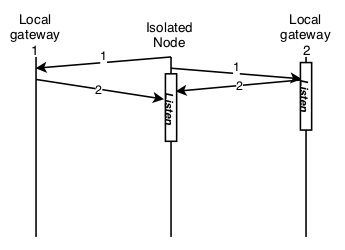
\includegraphics{discover.png}}
\caption{Discover Phase}
\label{fig1}
\end{figure}
Phase 1: Discovery 
Isolated nodes broadcast messages to discover(message 1) a Local Gateway. The end-nodes send messages every (X + random Integer) seconds. If a  Gateway receive a discovery message, the Local Gateway will accept (message 2 )and communicate to the end-nodes the communication slots.



\begin{figure}[htbp]
\centerline{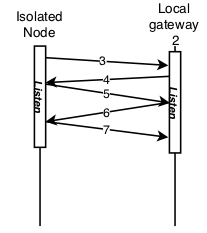
\includegraphics{register.png}}
\caption{Registering/pairing phase}
\label{fig2}
\end{figure}
Phase 2: Registration
 
The end-node will confirm the pairing to the Local gateway (message 3) . The end-node is registered to the Local gateway. 
There might be several Local gateway inside the system. However, there must never be multiple registrations on the same one.
After the local gateway receive the message 3, gateway send to the isolates node the message 4 to give his acknowledgment.
Message 5 is the first message from the isolated node, which contains datas to put an end the pairing phase. When all this stuff is done, the local gateway is able to send the message 6 : a request of data, then the node will answer his data.
 
\begin{figure}[htbp]
\centerline{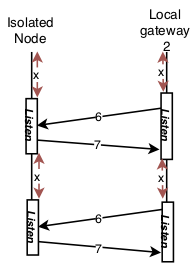
\includegraphics{harvest.png}}
\caption{harvest phase}
\label{fig3}
\end{figure}
Phase 3: Collection
The Local gateway will ask data to the end-nodes. If so, the isolated node sends the data to the Local gateway. This one will then forward it to another Gateway.
\subsubsection{Accuracy}
Each message contains information on the next slot, the time of listening on this one, as well as the id of the senders and receivers. If a message is lost or collapsed, it will be re-sent managed by timers.

\subsubsection{Particular case}
When two gateways are in range from the isolated node and there both answer to him with the message 2. The isolated node pick one randomly.
To manage multiple isolated node, 
\section{Algorithm and simulation}
\subsection{Algorithm}

\subsubsection{Messages format}

The set of system messages are of the form:

\begin{center}
\texttt{< message\_type , source , destination , data >}
\end{center}

There are several messages in the system. It is considered that each message corresponds to a function carrying the name of the message, initializing the type and the source of the message, and taking in parameter the destination and the data.

\subsubsection{Message from IN to GW}
\begin{itemize}
    \item The \texttt{discover} message
    \begin{itemize}
      \item message set up for the discovery of a \texttt{GW} by an \texttt{IN}
      \item \texttt{destination = udef} :  broadcast mode
      \item \texttt{data = udef} : nothing
    \end{itemize}
    \item  Messages \texttt{pair}
    \begin{itemize}
      \item Pairing message from an IN to a GW.
      \item \texttt{data = udef} : nothing
    \end{itemize}
    \item Messages \texttt{data\_response}
    \begin{itemize}
      \item Answer from the data request of a GW.
    \end{itemize}
\end{itemize}

\subsubsection{Messages from GW to IN}
For all the messages coming from the \texttt{GW} the data part is structured as follows:

\begin{itemize}
  \item \texttt{answer\_frequency} : frequency on which the IN must respond
  \item \texttt{next\_slot} : delay by the next listening window
  \item \texttt{next\_duration} : fixed time of the next listening window
  \item \texttt{next\_frequency} : Frequency of the next listening window
  \item \texttt{data} : data space specific to the exchange
\end{itemize}

The message is like that   :

\begin{center}
\texttt{< message\_type , source , destination , answer\_frequency , next\_slot , next\_duration , next\_frequency , data>}
\end{center}

The different messages \texttt {GW} $ \ rightarrow $ \texttt {IN} are thus:
\begin{itemize}
     \item the messages \texttt {candidate} 
     \begin {itemize}
       \item \ texttt {GW} reply message after receiving \texttt{discover} from \texttt{IN}
       \item \ texttt {data = udef}: no info
     \end{itemize}
     \item messages \texttt{data\_request}
     \begin{itemize}
       \item data request message
       \item \texttt{data = udef} if only one data available or \texttt{data = requested\_data} in the case of multiple data
     \end{itemize}
\end {itemize}

\subsubsection{List of differents used functions}

\paragraph{Sending functions}

\texttt{void send(frequency , message)}

\paragraph{Receiving functions}

The function will \texttt{listen}  on a particular \texttt{frequency} during time defined by \texttt{time} The function is decribed like this :

\begin{center}
\texttt{(message,time) listen(frequency , source , message\_type , time\_listen)}
\end{center}

the values of the parameters of this function are:
\begin{itemize}
  \item \texttt{frequency} : listening frequency
  \item \texttt{source} : id of the sender of the message
  \begin{itemize}
    \item \texttt{source = udef} : listen to all nodes on the defined frequency
  \end{itemize}
  \item \texttt{message\_type} : type of message expected
  \begin{itemize}
    \item \texttt{message\_type = udef} : listen to all types of messages  \end{itemize}
  \item \texttt{time\_listen} : duration of the reception window
  \begin{itemize}
    \item \texttt{time\_listen = udef} :  infinite window \end{itemize}
\end{itemize}

Return values are :

\begin{itemize}
  \item \texttt{message} message received
  \begin{itemize}
    \item passage of the message in its totality
        \item \texttt{message == udef} : no reception respecting the constraints
  \end{itemize}
  \item \texttt{time} remaining time based on \texttt{time\_listen}
  \begin{itemize}
    \item \texttt{time == udef} :in the case of \texttt{time\_listen = udef}
  \end{itemize}
\end{itemize}
\newpage

The subtlety to ensure that an isolated node is waiting for a request for data lies in the first data request message that contains the data: In how long I have to be awake and for how long I should be .
So once the data is sent and the end of the slot arrives the node goes to sleep again (if it's the first time it works) and wakes up in time to the next window of data request. There are two conditions for these to pass correctly.
\begin {itemize}
\item Firstly the rest time must be long enough, indeed if the relay has a lot of node to collect, if the time is not enough it can never be in deep sleep state and therefore can exhaust its battery.
\item Secondly the calculation of the slot sent in the request message. If there is once again a lot of node harvested for the relay. he must make sure to save the isolated nodes attached to him, he can calculate an offset corresponding to the order in which he will pick up the one he sends this slot value.
\end {itemize}
\begin{algorithm}[!h]
\caption{Initialization of communication variables of IN}\label{alg:intvar}
\begin{algorithmic}[1]
\Procedure{$init\_var$}{msg}
\State $gw \leftarrow msg.source$
\State $next\_time \leftarrow msg.next\_slot$
\State $timer \leftarrow msg.next\_duration$
\EndProcedure
\State
\Procedure{$flush\_var$}{~}
\State $gw \leftarrow udef$
\State $msg \leftarrow udef$
\State $next\_time \leftarrow udef$
\State $timer \leftarrow timer\_disco$
\EndProcedure
\end{algorithmic}
\end{algorithm}
\begin{algorithm}
\caption{Algorithm IN 1-1}\label{alg:in1-1}
\begin{algorithmic}[1]
\While{$(true)$}
  \State $flush\_var()$
  %\State \Comment{------------------------------------------------------- \textit{phase d'apairage}}
  \While{$(msg = udef)$}
    \State $send(freq\_listen,discover(udef,udef))$
    \State $(msg,t) = listen(udef,candidate,timer +rnd())$
  \EndWhile
  \State $initVar(msg)$
  \State $send(freq\_send,pair(gw,udef))$
  \State
  %\State \Comment{----------------------------------------------\textit{Phase d'échanges}}
  \While{$(gw != udef)$}
    \State $sleep(next\_time)$
    \State $(msg,t) = listen(gw,data\_request,timer)$
    \If{$msg != udef$}
      \State $initVar(msg)$
      \State $send(fdate\_response(gw,local\_data)$
    \Else
      $flush\_var()$
    \EndIf
  \EndWhile
\EndWhile
\end{algorithmic}
\end{algorithm}

\begin{algorithm}
\caption{Initialization of communication variables of GW}\label{alg:initvarlg}
\begin{algorithmic}[1]
\Procedure{$init\_var$}{~}
\State $freq\_send \rightarrow chose()$
\State $timer \leftarrow chose()$
\State $freq\_listen \leftarrow chose()$
\State $freq\_next \leftarrow chose()$
\EndProcedure
\State
\Procedure{$flush\_var$}{~}
\State $timer \leftarrow timer\_disco$
\State $freq\_listen \leftarrow freq\_disco$
\State $freq\_send \leftarrow freq\_disco$
\State $in \leftarrow udef$
\EndProcedure
\end{algorithmic}
\end{algorithm}

\begin{algorithm}[H]
\caption{Algorithm gw 1-1}\label{alg:gw1-1}
\begin{algorithmic}[1]
\State $flush\_var()$
\While{$(true)$}
  \If{$(in == udef)$}
    \State $(msg,t) = listen(,udef,discover,timer)$
  \EndIf
  \If{$(msg != udef)$}
    \State $in \leftarrow msg.source$
    \State $init\_var()$
    \State $send(candidate(in,slot,duration,udef)$
    \State $(msg,t) = listen(,in,pair,timer)$
    \If{$(msg == udef)$}
      \State $flush\_var()$
    \EndIf
  \EndIf
  \If{$(in != udef)$}
    \State $init\_var()$
    \State $send(data\_request(in,slot,durationt,udef)$
    \State $(msg,t) = listen(in,data\_response,timer)$
    \If{$(msg != udef)$}
      \State $send\_data(id + ":" + local\_data + ";" + in + ":" + msg.data)$
    \Else
      \State $send\_data(id + ":" + local\_data + ";" + in + ":" + udef)$
      \State $flush\_var()$
    \EndIf
  \EndIf
\EndWhile
\end{algorithmic}
\end{algorithm}
\subsection{Simulation}
 We simulated 100 graphs with each 1000 nodes and for each configuration:
\begin{itemize}
\item Variation of the number of nodes isolated by gateway between 1 to 4.
\item Variation of the maximum gateway number per well between 1 to 4.
\item Variation of the number of data to recover per day between 1 and 24 messages.
\item Variation on the method of reassembly of the data collected by the isolated nodes (ie, sent to the well at each reception (NA method) or reassembled after merging of all the messages  (A method) )
\item Variation of the speed of each link between two nodes.
\end{itemize}
Which makes us a total of 12800 graphs to create. In order to realize this creation we have written an algorithm based on the probability of existence of a link between two nodes.That is to say that at the beginning we create the first well. At that one looks at its degree (which is zero at the beginning) of gateway hooked to it. One draws a probability and if it is greater than that established in input of the algorithm one adds a gateway and the link between the well and this one. We do the same with the isolated nodes.
In order to summarize we had:
one hundred graphs with a maximum of one isolated node per gateway and a maximum of one gateway per well. This configuration will be abbreviated 1 (IN) -1 (GW) $\rightarrow$ 1-1. 

So we used the Omnet ++ tool to simulate all these graphs and each case. In these we have noted for isolated node the number of messages sent as well as the remaining battery at the end of the simulation.
For the battery we assumed that it had 6600 mAh or 23760000 mAs. The consumed electric energy was taken from the LoPy documention, WiFi section. Our forecast calculations are realized as follows:

The device is considered to send X msg (\#msg) per day (over 24 hours). The current of an emission is Ce = 107.3 mA. Each emission lasts Te = 2s.
The current in reception is Cr = 37mA. The time in reception is Tr
The standby current is Cv = 0.531 mA. The device is idle for Tv = (24 * 3600- \#msg * Te-Tr * Cr)
The current consumed on a day is therefore:
CDay (mA.s) = (\#msg * This * Te + Cr * Tr + Cv * Tv)

So here is a graph showing the difference between aggregation and non-aggregation mode at the message level. 
\begin{figure}[htbp]
\centerline{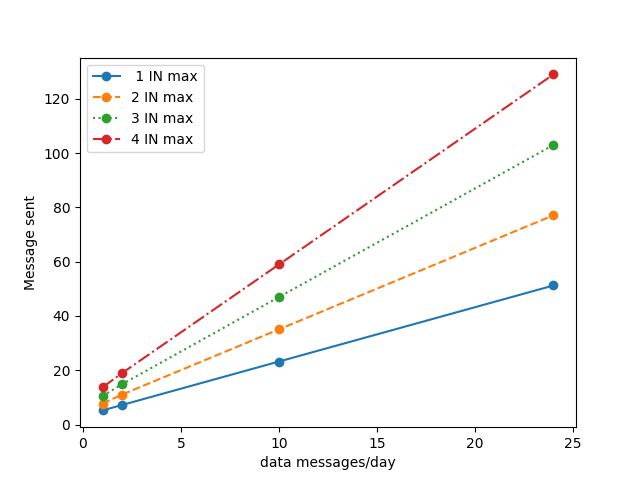
\includegraphics[scale=0.5]{graphics_resultats/A/A.png}}
\caption{Mode : Agregation}
\label{A}
\end{figure}
We can notice that in the following figures that a linear aspect stands out clearly on the variation of the number of messages on the part of a gateway whatever the mode (with aggregation or without aggregation).
\begin{figure}[htbp]
\centerline{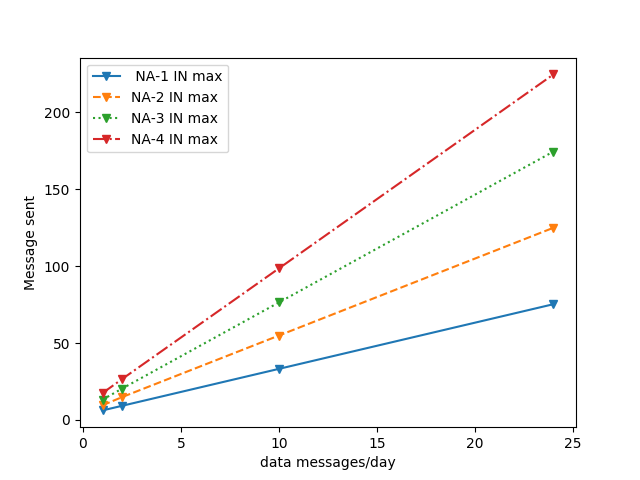
\includegraphics[scale=0.5]{graphics_resultats/A/NA.png}}
\caption{Mode : No agregation}
\label{A}
\end{figure}
What we can also notice is the number that as expected is bigger and grows much faster without the aggregation mode ( Fig 4, 5, 6).
What can therefore be considered significant enough. This is because adding the data of the gateway to those of the isolated nodes makes the number of messages in cluster mode to the same numbers as if the INs were GWs and thus connected nodes.
\begin{figure}[htbp]
\centerline{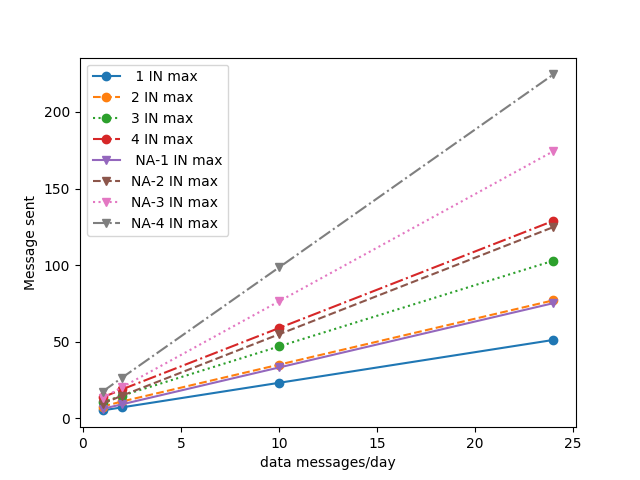
\includegraphics[scale=0.5]{graphics_resultats/A/AvsNA.png}}
\caption{Mode : Agregation vs No Agregation}
\label{A}
\end{figure}

The objective was to check if the intuitive idea is right: the architecture with intermediary relay and aggregation returns, in number of messages and thus lifespan of the network, to the model without relay, the model or each client speaks live with antennas always UP.

Figures 7 to 10 are more complex. Indeed these graphs represent by their colors the number of maximum Gateway related to a well. Each point is a simulation recall described by the maximum degree of gateways and isolated nodes as well as the number of messages requested by the well per day. Here these four figures are in aggregation mode.

First on each graph, each point is an average of the number of messages sent or the state of the battery if any, by an isolated node, or by a gateway if necessary. For each graph, the block of 4 colors is therefore the set of graphs with degree 1 IN. it should be understood that the simulations from 0 to 399 are those called "1-1, 1-2, 1-3, 1-4". from 400 to 799 "2-1, 2-2, 2-3, 2-4" etc.
We realized these simulations with as previously said a number of message requested by the different well. Indeed we chose: 1, 2, 10, 24 messages per day.
\begin{figure}[htbp]
\centerline{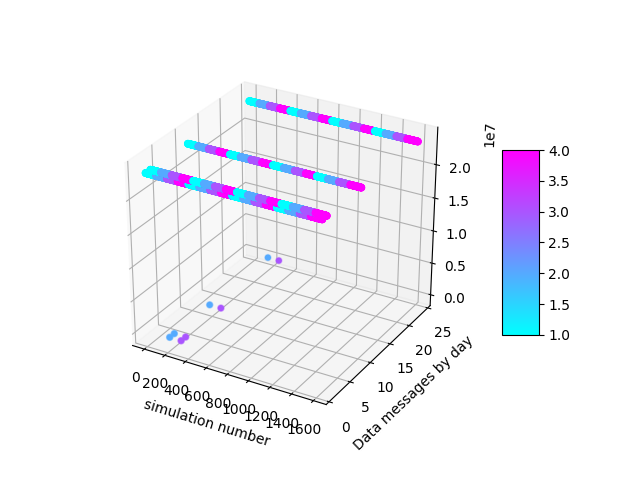
\includegraphics[scale=0.5]{graphics_resultats/bat/Sim_MSG_SEND_data_bat_gw_degree_gw.png}}
\caption{State of the battery on a Day / data message required/day for a gateway}
\label{A}
\end{figure}

\begin{figure}[htbp]
\centerline{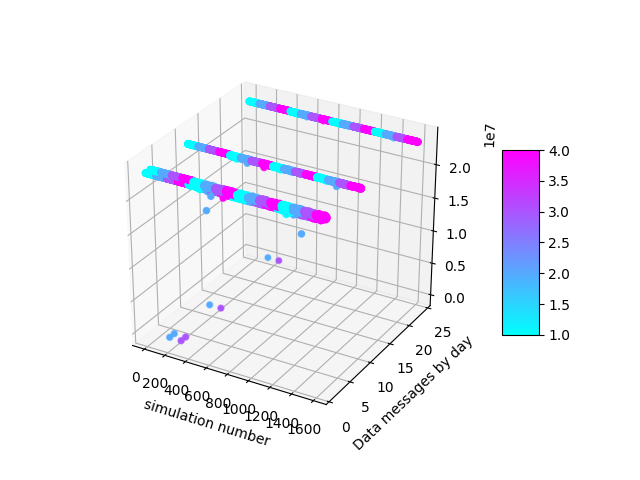
\includegraphics[scale=0.5]{graphics_resultats/bat/Sim_MSG_SEND_data_bat_in_degree_GW.png}}
\caption{State of the battery on a Day / data message required/day for an IN}
\label{A}
\end{figure}


\begin{figure}[htbp]
\centerline{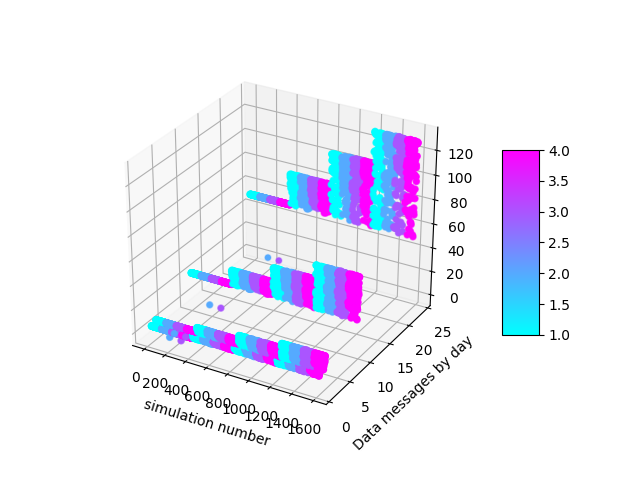
\includegraphics[scale=0.5]{graphics_resultats/msg/Sim-MSG_GW-MSG_SEND-degree_GW.png}}
\caption{Number of message on a Day / data message required/day for a gateway}
\label{A}
\end{figure}
The previous remark made on the message number which remains coherent with respect to an architecture without relays it also on the state of the battery on the side of the isolated nodes, from the moment when the pairing is carried out.
Of course, in the different figures such as FIG. 10 or FIGS. 8 and 7, there are very distinct points of all the others, these can be explained by a set of things:
\begin {itemize}
\item The connection / link is too bad / noisy so the device may have fallen out of battery / have sent too many messages. and therefore can never be recognized across the entire network.
\item Corruption on identifiers.
\item bad calibration of the device on its WiFi antenna
\end {itemize}
\begin{figure}[htbp]
\centerline{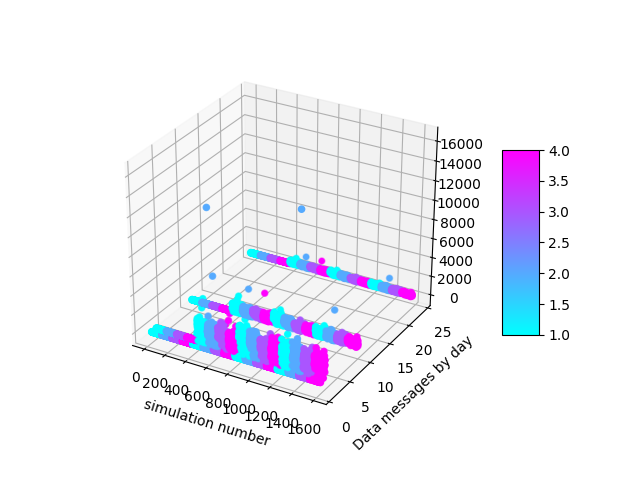
\includegraphics[scale=0.5]{graphics_resultats/msg/Sim-MSG_IN-MSG_SEND-degree_GW.png}}
\caption{Number of message on a Day / data message required/day for an IN}
\label{A}
\end{figure}


\newpage
\section{Conclusion}

To conclude, we have therefore shown that it is possible to rally isolated nodes directly by the network concealer in order to retrieve despite all the data it has. All with a proof that the number of messages does not explode in aggregation mode compared to an architecture where the nodes would be connected directly to the hubs. The battery therefore remains in the same state whatever the architecture from the moment the pairing is done.
We've also seen how to make sure a node is awake and waiting to send that data to its relay.
It is expected to know how to handle the system once pairing is complete when an error / problem occurs. For example, what happens if the relay goes down? How to detect it from the IN and the well? How to know that an IN has failed from a gateway?




\cite{Tanaka2018},
\cite{Singh2012},
\cite{Ng2013},
\cite{Palan2017},
\cite{Sharma2006},
\cite{Haddad2009}
\section*{Acknowledgment}


\bibliographystyle{plain}
\bibliography{article}
%\bibliography{article} 
%\bibliography{sample} 
\end{document}
